Las cuencas se delimitaron con direcciones de flujo calculadas por el método de ocho direcciones (D8) sobre FABDEM reproyectado al sistema UTM, huso 19 sur (datum WGS~84), con celdas de \SI{30}{m}. Una delimitación preliminar en coordenadas geográficas subestimaba el área. La salida de cada cuenca es la celda de máxima acumulación a menos de \SI{120}{m} del punto donde el cauce cartografiado entra a la urbanización. Resultan H1 con \SI{8,04}{km^2} y un relieve de \SI{1376}{m}, S1 con \SI{1,90}{km^2} y S2 con \SI{0,17}{km^2}: en total, \SI{10,1}{km^2} aportantes.

Se usaron dos estimaciones independientes, que no se combinan en una sola distribución:
\begin{itemize}
\item \textbf{Balance lluvia--escorrentía con agua y sólidos diferenciados:} $V_w=f_wPAC$ y $V_m=V_w/(1-\Cvt)$, donde $V_w$ es el volumen de agua incorporado al pulso; $P$, la precipitación acumulada; $A$, el área de la cuenca; $C$, el coeficiente de escorrentía; $f_w$, la fracción de escorrentía incorporada al pulso; y $V_m$, el volumen de mezcla. Los rangos son: precipitación del pulso del evento $P$ entre \SI{12}{\milli\metre} y \SI{35}{\milli\metre}, $C\in[0{,}3;0{,}8]$, $f_w\in[0{,}5;1]$ y $\Cvt\in[0{,}30;0{,}50]$.
\item \textbf{Modelo empírico para cuencas quemadas} \citep{gartner2014}, aplicado por subcuenca e incluyendo su error residual $\varepsilon\sim N(0;1{,}04^2)$. Ese modelo predice el volumen de depósito $V_\mathrm{dep}$, que se convierte a volumen de mezcla con $V_m=(1-\phi)V_\mathrm{dep}/\Cvt$, donde $\phi$ es la porosidad del depósito. Su aplicabilidad fuera del sur de California es una hipótesis.
\end{itemize}
Las distribuciones se resumen mediante la mediana y los percentiles 5 y 95, y el caudal pico correspondiente se estima con la relación de \citet{mizuyama1992}. La calibración recorre volúmenes de \SI{80000}{\metre\cubed} a \SI{300000}{\metre\cubed}. Los resultados iniciales se presentan en la sección~\ref{sec:res-volumen}; la actualización con severidad estimada por dNBR, en la sección~\ref{sec:res-incendio}.

\begin{figure}[htbp]\centering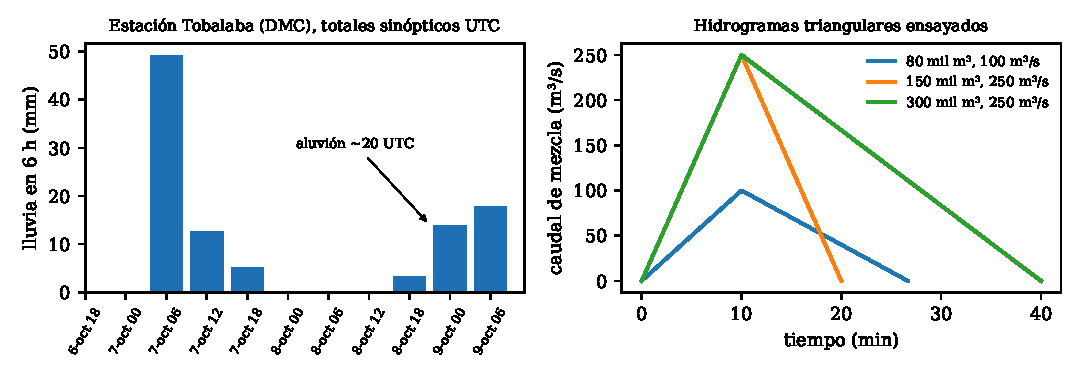
\includegraphics[width=\textwidth]{forzamiento}\caption{Forzamiento observado y supuesto del modelo. Izquierda: lluvia acumulada cada \SI{6}{h} en la estación Tobalaba de la Dirección Meteorológica de Chile \citep{dmc2026} entre el 6 y el 9 de octubre de 2026 (horas UTC; la prensa citada en el relato sitúa el aluvión hacia las 20 UTC del 8 de octubre). Derecha: hidrogramas triangulares de mezcla ensayados.}\label{fig:forzamiento}\end{figure}

\paragraph{Escenario de suelo saturado.} Con la información hidrometeorológica conocida después del cribado (sección~\ref{sec:evidencia}) se agregó una tercera estimación, tampoco combinada con las anteriores. La relación entre la isoterma informada y la cota máxima de la cuenca (\SI{2355}{m}, igual a la que informa el CR2; una versión previa del texto indicó por error \SI{2775}{m}, cifra que no se usó en ningún cálculo: la delimitación D8 y la hipsometría siempre se basaron en la cota del modelo de elevación) sustenta el supuesto de precipitación líquida sobre toda el área aportante, y la saturación del suelo informada por la autoridad se adopta como supuesto del escenario de cálculo. Se usan $P\in[20;40]$~\si{mm}, $C\in[0{,}6;0{,}9]$ y $f_w\in[0{,}6;1]$. El aporte por fusión de nieve se acota por arriba con \SI{50}{mm} de equivalente en agua sobre los \SI{0,31}{km^2} de la cuenca situados sobre \SI{2000}{m}.
